%!TEX root = ../article.tex

% A new section
\section{Solution}
\label{sec:solution}


\subsection{Overview}
We set out to create an \gls{ide} for \gls{gd} programming that is available as a web application.
To do that, we identified several tasks that the programming environment needs to support in order to be useful for the architect.
It needs to:
(1) let the architect develop programs;
(2) run programs;
(3) display their results;
(4) make it easy to understand programs;
and (5) export results to the most used commercial \gls{cad} applications.

To accomplish these tasks, there are two separate components, as seen in Figure~\ref{fig:archi:sol}: (1) the web application, that supports the \gls{ui} for creating programs;  and (2) the remote CAD application, that offers an \gls{api} for running programs in \gls{cad} applications.
The first four tasks can be handled by the web application alone since there is no need to interact with the \gls{cad} applications running in the user's computer.
The forth task requires both the web application and the remote CAD service.

We made a test implementation of this architecture which we will call Luna Moth from here on.
In the rest of the section, we describe these two components and how each of the tasks is implemented in Luna Moth.

We start by looking at the web application.

\begin{figure}
  \centering
  \includegraphics[width=1.0\linewidth]{./\figurePath/architecture_overview/architecture_overview}
  \caption{Architecture of the solution.}
  \label{fig:archi:sol}
\end{figure}


\subsection{Web application}
To handle the tasks of letting the architect develop programs, running programs, supporting program understanding, and displaying results, Luna Moth's \gls{ui} has the layout shown in Figure~\ref{fig:page:view}.
Taking up most of the screen space are a text editor (C) and a 3D view (D) that allow the architect to edit a program and view its results.
On top of the text editor and the 3D view are controls for the running process (B), including whether to run automatically and whether to collect data to display traceability.
On the left are hidden panels for actions like selecting a program and exporting to \gls{cad} applications (A).

\begin{figure}
  \centering
  \includegraphics[width=1.0\linewidth]{./\figurePath/webpage_view/webpage_view}
  \caption{Layout of Luna Moth's \gls{ui}.}
  \label{fig:page:view}
\end{figure}


\subsubsection{Program Comprehension}
In \gls{gd}, the architect interacts with the program that creates the model instead of creating it directly in a \gls{cad} application.
This allows him to automate tasks that normally take too much time and, therefore, also allows him to explore a design space with much more complexity.
However, since he is not directly interacting with the model, he needs to understand the relationship between the program and its results in order to know how to change the program to get the model he wants.
The process of understanding the program and how it relates to its results is called program comprehension\cite{rugaber1995program}.
Luna Moth enables him to do this by providing immediate feedback to changes and by showing traceability.


\paragraph{Adjusting Literals}
When a value, such as a number, is typed directly into a program’s source code, it is called a literal value, or simply literal.
When using \gls{gd}, architects find themselves repeatedly adjusting these literals to tweak the generated model.
This is usually done by rewriting parts of the literal’s text with higher or lower digits and, then, re-running the program to see the effect.

However, editing literals this way often leads to errors, since it is easy to mistype characters.
The architect can increase the literal's value by an order of magnitude if, by mistake, he inserts one character without removing another.
Furthermore, when increasing the literal in steps, different hand movements are required when the increment results in a carry over, e.g. when going from ninety-nine to one hundred, yet again increasing both the likelihood of mistyping and the time it takes to make the changes.

These mistakes get amplified when the programming environment provides real-time feedback and, like so, begins rerunning the program before the error is corrected, thus leading to reduced \gls{ui} responsiveness.
The adjustment can be friendlier if done in a clearer way instead of retyping the literal, Luna Moth enables the adjustment by simply ``clicking and dragging'', a movement that is similar to a ``slider''.

\begin{figure}
  \centering
  \begin{subfigure}[b]{0.49\linewidth}
    \includegraphics[width=1.0\linewidth]{./\figurePath/literal_adjustment/2_start_crop_big}
  \end{subfigure}%
\hspace{0.01\linewidth}%
  \begin{subfigure}[b]{0.49\linewidth}
    \includegraphics[width=1.0\linewidth]{./\figurePath/literal_adjustment/2_end_crop_big}
  \end{subfigure}
  \caption{Example of literal adjustment.}
  \label{fig:lit:adjust}
\end{figure}


\paragraph{Traceability}
Reducing the time between making a change and seeing its effect is one way to help the architect to understand a program.

Another way to understand the program is to understand the relationship between parts of the program and parts of the results.
If the programming environment takes care of tracking the relation between the program and results, the architect only needs to ask for the relation instead of having to track it by himself, freeing his mind to think about the problem.

There needs to be a way to give the architect quick access to the relation being tracked by the environment.
To do this, Luna Moth highlights certain parts of the program and its results when the pointer is on either one.
More specifically, when the pointer is over a part of the program, it highlights all the results that it produced;
when the pointer is over a part of the results, it highlights the part of the program where it was created.
Figure~\ref{fig:trace:example} shows an example for both of this cases.

Currently, Luna Moth only tracks the results produced by calls to functions.
This was a compromise to balance performance, since keeping track of traceability is an additional task that needs to be performed while running the program.

\begin{figure}
  \centering
  \begin{subfigure}[b]{1.0\linewidth}
    \includegraphics[width=1.0\linewidth]{./\figurePath/traceability_example/code_to_results_crop}
    \caption{From code to results.}
    \label{sub:code:to:results}
  \end{subfigure}

  \begin{subfigure}[b]{1.0\linewidth}
    \includegraphics[width=1.0\linewidth]{./\figurePath/traceability_example/results_to_code_crop}
    \caption{From results to code.}
    \label{sub:results:to:code}
  \end{subfigure}
  \caption{Two examples of the traceability mechanism. The first from program to results and the second from results to program.}
  \label{fig:trace:example}
\end{figure}


\subsubsection{Running Programs}
One of the fundamental parts of the programming environment is that it runs programs.
To run programs, the environment needs to support a programming language.
This includes the syntax and semantics of the language and the primitive operations that are available to programs.
After knowing these, the environment must implement a process to run the program and collect results so as to display them later.


\paragraph{Program Structure}
Before a program can be run, the programming language has to be defined.
In Luna Moth, we decided that it would be best to use JavaScript, as it was thought for designers and also because of its current performance in modern web browsers.

In addition to the programming language, the environment also needs to get results from programs.
Luna Moth uses the values of the top-level expression statements of the program as its results.


\paragraph{Running process}
When Luna Moth runs a program, it needs to do two things: (1) collect the results of the program; and (2) collect traceability data.
It does these two by instrumenting the program with additional calls to special functions that record the desired information.

To be able to perform the instrumentation, Luna Moth parses the program using Esprima, a JavaScript parser,\footnote{https://github.com/jquery/esprima (last accessed on 10/05/2017)} to get its \gls{ast}.%
\footnote{The \gls{ast} conforms to a community standard. It can be found at https://github.com/estree/estree (last accessed on 10/05/2017).}

Afterwards, the \gls{ast} is transformed by adding a recording call to (1) all top-level expression statements and (2) all function call expressions.
Figure~\ref{fig:instrument:example} exemplifies the transformation.
To let the recording functions know what top-level expression or function call is producing a result, we also provide them with identifiers for those expressions.

After this step, Luna Moth creates a new function with the instrumented program as its body.
The primitives and recording functions are provided as parameters to this new function.

Finally, the newly created function is called and, afterwards, the recorded information is made available to the rest of the system.

\begin{figure}
  \centering
\begin{minipage}[t]{1.0\linewidth}
  \begin{minted}[frame=lines]{js}
let s = sphere.byRadius(5);
s;




  \end{minted}
\center{Before}
\end{minipage}
%\hspace{0.05\linewidth}
\center{\rule{0.8\linewidth}{0.4pt}}
\begin{minipage}[t]{1.0\linewidth}
  \begin{minted}[frame=lines]{js}
let s = recordCallResult(
   sphere.byRadius(5),
   /*function call ID*/);
recordTopLevelResult(
   s,
   /*top-level expression ID*/);
  \end{minted}
\center{After}
\end{minipage}
  \caption{A program before and after the transformation.}
  \label{fig:instrument:example}
\end{figure}


\subsection{Remote CAD Service / Exporting to CAD}
The last task that Luna Moth needs to support is exporting to the most used commercial \gls{cad} applications.
As opposed to the other tasks, exporting to a \gls{cad} application requires the web page to communicate with other applications.
Unfortunately, web pages are not allowed to communicate with applications running in the computer displaying them.

To make communication possible, Luna Moth includes an application, the \textit{remote CAD app}, that the architect must install and run in his computer when he wants to export results.
This application serves as a bridge between \gls{cad} applications installed in the computer and the environment running on the web browser.
After being started, the application detects which \gls{cad} applications are installed in the computer and connects to the \textit{environment directory} so it can be discovered by the web application.
When the architect needs to export a program to his \gls{cad} application, the environment connects to the application in his computer through the \textit{environment directory} and starts to send requests to it, in order to create shapes in the \gls{cad} application.

Figure~\ref{fig:remote:cad:example} shows an example of the export to \gls{cad} functionality.
The architect has created a program using Luna Moth.
After selecting AutoCAD and SketchUp as export destinations, he starts the export process and, afterwards, the model resulting from running the program is available in both \gls{cad} applications.

\begin{figure}
  \centering
  
\includegraphics[width=1.0\linewidth]{./\figurePath/remote_cad_example/remote_cad_example}
  \caption[An example of the remote CAD service.]{An example of the remote CAD service. The results of the program have been passed to both AutoCAD and SketchUp.}
  \label{fig:remote:cad:example}
\end{figure}
